%%%%%%%%%%%%%%%%%%%%%%%%%%%%%%%%%%%%%%%%%%%%%%%%%%%%%%%%%%%%%%%%%%%%%%%%%%%%%%%%
\chapter{Постановка задачи и выбор пути решения}
%%%%%%%%%%%%%%%%%%%%%%%%%%%%%%%%%%%%%%%%%%%%%%%%%%%%%%%%%%%%%%%%%%%%%%%%%%%%%%%%

В данном разделе рассматриваются основные требования, предъявляемые к методу обнаружения клонов. Приводится постановка и подробное описание задач, решаемых в рамках данной работы, в том числе:
\begin{itemize}
\setlength\itemsep{0mm}
\item задача разработки метода обнаружения клонов, основанного на использовании искусственных нейронных сетей
\item задача разработки прототипа инструмента обнаружения
\end{itemize}
%%%%%%%%%%%%%%%%%%%%%%%%%%%%%%%%%%%%%%%%%%%%%%%%%%%%%%%%%%%%%%%%%%%%%%%%%%%%%%%%
\section{Задача разработки интеллектуального метода обнаружения клонов}
%%%%%%%%%%%%%%%%%%%%%%%%%%%%%%%%%%%%%%%%%%%%%%%%%%%%%%%%%%%%%%%%%%%%%%%%%%%%%%%%

Целью данной работы является разработка метода для обнаружения клонов. Главное требование, которое предъявляется к разрабатываемому методу - использование искусственных нейронных сетей. Кроме того, разрабатываемый метод интеллектуального обнаружения клонов должен обеспечивать решение следующих задач:
\begin{itemize}
\setlength\itemsep{0mm}
\item обнаружение клонов I-III типов;
\item максимизация полноты и точности обнаружения;
\item извлечение информации о клонах в виде клоновых классов.
\end{itemize}

Несмотря на тот факт, что разрабатываемый метод должен быть интеллектуальным, в качестве предварительной обработки необходимо привести исходный код к одному из подходящих видов внутреннего представления. В предлагаемом подходе было решено использовать несколько представлений (гибридный метод). Этими представлениями являются AST и последовательность токенов. 

Использование AST позволяет сохранить информацию о структуре исходного текста программы, именно благодаря этому становится возможным увеличить полноту и точность результатов.

Использование токенов в качестве представления исходного кода позволяет, в свою очередь, значительно сократить размер входных данных.

Общую структуру внутреннего представления кода можно увидеть на рис.~\ref{fig:stages}

\begin{figure}[htbp]
\centering
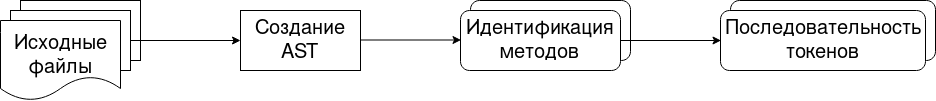
\includegraphics[width=\textwidth]{stages.png}
\caption{Структура внутреннего представления кода}
\label{fig:stages}
\end{figure}

\section{Задача разработки прототипа инструмента}

Одна из задач данной работы заключается в разработке и тестировании прототипа на базе предложенного метода. Учитывая выбранный подход, задача реализации прототипа состоит из двух частей:
\begin{enumerate}
\item Разработка инструмента, производящего преобразование исходного кода в выбранное представление;
\item Разработка инструмента, использующего нейронные сети для поиска клонов.
\end{enumerate}

\subsection{Разработка инструмента для создания внутреннего представления}

К разрабатываемому инструменту предъявляются следующие требования:
\begin{itemize}
\setlength\itemsep{0mm}
\item получение исходного кода на языка Java из заданной директории
\item построение AST для полученного кода
\item фильтрация AST
\item преобразование AST в последовательность токенов
\end{itemize}

В качестве целевого языка был выбран язык Java, так как на протяжении многих лет он является одним из самых распространенных и используемых языков программирования (согласно TIOBE)~\cite{TIOBE}. 

\subsection{Разработка инструмента для поиска программных клонов}

Вторая важная часть разработки прототипа - реализация инструмента поиска клонов. К такому инструменту предъявляются следующие требования:
\begin{itemize}
\setlength\itemsep{0mm}
\item использование рекуррентных нейронных сетей для поиска клонов
\item поиск клонов I-III типов
\item высокая точность и полнота поиска
\end{itemize}

Для данного инструмента, в качестве целевого языка программирования был выбран язык Python. Такой выбор был сделан из-за популярности и частым использованием его в области разработки нейронных сетей. К тому же, для данного языка программирования существует множество библиотек для реализации и обучения нейронных сетей. Одна из них - Tensorflow, которая и была использована в данной работе~\cite{tf}.
